\chapter{\TLA}
\label{cap2}

\TLA é uma linguagem de especificação de software, criada por Leslie Lamport \cite{tlahistory} voltada à modelagem de sistemas concorrentes. Ela se propõe a oferecer uma maneira mais simples de escrever um algoritmo, ao utilizar um nível de abstração acima do que há ao escrever código em uma linguagem de programação. Assim, ao programar, não é necessário atentar-se a detalhes de implementação, permitindo o foco no comportamento do algoritmo - e não das suas dependências.

As especificações são descritas em fórmulas lógicas, com pequenas adaptações de sintaxe. Para facilitar a curva de aprendizado para engenheiros, foi criada a linguagem PlusCal \cite{pluscal}, com uma sintaxe semelhante a linguagens de programação imperativas, e que traduz seus programas para \TLA. A linguagem PlusCal não permite especificar sistemas tão complexos quanto os que podem ser escritos diretamente em \TLA, mas, devido à tradução para a linguagem original, aproveita completamente as capacidades dela de verificação de propriedades.

O método de especificação é baseado em máquinas de estados \cite{tlahistory} e, sendo assim, a descrição de um modelo é composta por uma condição inicial, que determina os possíveis estados inciais, e por uma relação de transições, que determina os possíveis estados que podem suceder cada estado em uma execução. Dessa forma, o conjunto de comportamentos especificado é composto por todos os comportamentos cujo estado inicial satisfaz a condição inicial e todas as transições fazem parte relação.

Lamport destaca \cite{hyperbook} que as especificações deveriam ser sobre modelos de uma abstração do sistema, e não algo retirado do próprio sistema. Semelhante à planta de um edifício, a especificação pode ser consultada para obter informações sobre o edifício (ou programa) de forma mais conveniente, além de ser capaz de facilitar uma série de verificações e perceber problemas enquanto a mudança ainda não é inviavelmente custosa.

Sendo assim, uma especificação em \TLA pode ser sobre comportamentos do ambiente no qual o programa funciona - como ao especificar um sistema e verificar possíveis comportamentos indesejáveis, entendendo aonde o programa deve atuar - descrevendo as operações existentes daquele sistema.

Não limitada a definição de um sistema, uma especificação pode incluir comportamentos do programa em si, compostas por operações existentes do sistema e novas operações definidas pelo programa. Em seu livro \cite{specifying-systems}, Lamport define um sistema de memória linear e, então, propõe uma implementação de um programa de escrita através de \textit{cache} que atua sobre um sistema de memória linear. Assim, ele verifica que a especificação da implementação dele satisfaz a especificação do sistema e prova a implementação. Nos exemplos deste capítulo, serão explicadas especificações de sistemas e de implementações.

\section{Lógica Temporal}

\TLA combina a Lógica Temporal das Ações, TLA (\textit{Temporal Logic of Actions}), proposta por Lamport em \cite{tlaformalization}, com teoria dos conjuntos - mais especificamente, a teoria de conjuntos de Zermelo-Fraenkel (ZFC), como detalhado em \cite{merzlogic}.

Lamport sumariza em \cite{proofsystem} o uso de TLA em \TLA. TLA é uma lógica temporal linear. Em \TLA, as variáveis rígidas do TLA são chamadas constantes, enquanto as flexíveis são chamadas variáveis. As expressões podem ser construídas em lógica clássica de primeira ordem, e são denominadas operadores constantes. Uma função de estado é uma expressão construída de operadores constantes, constantes e variáveis. Por fim, as fórmulas não temporais construídas a partir de operadores constantes, constantes, variáveis e expressões sobre uma função de estado são denominadas ações - correspondendo a \textit{actions} em TLA.

Com essa estrutura, toda a complexidade das definições estão nas fórmulas de ações. Os operadores temporais são usados somente no momento de verificar propriedades de segurança, vivacidade e razoabilidade (\textit{fairness}).

Uma fórmula em TLA é verdadeira ou falsa em um comportamento, que é definido por uma sequência infinita de estados. Uma fórmula é dita válida se e somente se ela é verdadeira para todos os comportamentos. Uma especificação $F$ implementa outra especificação $G$ se e somente se qualquer sistema que satisfaz $F$ também satisfaz $G$, ou seja, a fórmula $G \implies F$ é válida.

Aos operadores de TLA, são atribuídos os seguintes significados \cite{tlaformalization}:
\begin{itemize}
  \item \ENABLED \FANCYA para uma ação \FANCYA é um predicado que é verdadeiro para um estado se e somente se é possível fazer um passo \FANCYA partindo daquele estado.
  \item Um predicado $P$ deve ser verdadeiro para os valores das variáveis definidas no estado inicial de um comportamento para ser satisfeito por ele.
  \item A fórmula $\square [\FANCYA]_f$ para uma ação $\FANCYA$ é satisfeita por um comportamento se e somente se cada passo do comportamento satisfaz \FANCYA ou mantém os valores de $f$.
  \item $\square F$ ($F$ é sempre verdadeiro) para uma fórmula TLA $F$ é satisfeito por um comportamento se e somente se $F$ é verdadeiro para todos os sufixos do comportamento.
  \item \EE $x : F$ para uma variável $x$ e uma fórmula TLA $F$ é satisfeito por comportamento se e somente se existem alguns valores a serem atribuído a $x$ que produzem um comportamento que satisfaz $F$. Esse operador é uma especialização do quantificador existencial comum $\E$ porque ele asserte a existência de uma sequência infinita de valores para $x$, e não um único valor.
  \item $WF_f (\FANCYA)$ -- Razoabilidade fraca (\textit{Weak fairness}) de \FANCYA -- para uma função de estado $f$ e uma ação \FANCYA é satisfeita por um comportamento se e somente se \FANCYA $\land (f' \neq f)$ é infinitamente não ativo ou infinitos passos \FANCYA $\land (f' \neq f)$ ocorrem.
  \item $SF_f (\FANCYA)$ -- Razoabilidade forte (\textit{Strong fairness}) de \FANCYA -- para uma função de estado $f$ e uma ação \FANCYA é satisfeita por um comportamento se e somente se \FANCYA $\land (f' \neq f)$ ocorre finitas vezes ou infinitos passos \FANCYA $\land (f' \neq f)$ ocorrem.
  \item $F \stackrel{+}\rightarrow G$ para fórmulas temporais $F$ e $G$ é verdadeiro para um comportamento se e somente se $G$ é verdadeiro, pelo menos, enquanto $F$ é.
  \item $\Diamond F$ (Eventualmente F) é definido como $\neg \square \neg F$.
  \item $F \leadsto G$ (Em qualquer momento em que $F$ for verdadeiro, $G$ eventualmente será) é definido como $\square(F \implies \Diamond G)$
\end{itemize}

 Além deles, existem os operadores lógicos $\land,\ \lor$ e $\neg$ com seus significados padrões.

As fórmulas não temporais são chamadas também de fórmulas transicionais. Na notação de \TLA, elas devem ser escritas entre colchetes e sucedidas por uma definição do conjunto de variáveis para o qual são permitidos passos balbuciantes (\textit{stuttering steps}) - passos nos quais nenhuma variável dentro do conjunto tem seu valor alterado.

%% CHOOSE IF CASE EXCEPT

\section{Exemplo 1 - Jarros de Água}

Para exemplificar uma especificação de um sistema, é possível definir um problema combinatório simples como o dos jarros de água. Nesse problema, são fornecidos dois jarros inicialmente vazios, um com capacidade de 3 litros e outro com capacidade de 5 litros, assim como uma fonte inesgotável de água. Sendo assim, é possível despejar a água dos jarros no chão, transferir a água de um jarro ao outro ou encher um jarro com a fonte de água.

O objetivo do problema é ter exatamente 4 litros de água em um dos jarros. Isso é, dada uma máquina de estados, é necessário encontrar uma sequência de transições que leva a algum estado onde o jarro maior tem exatamente 4 litros de água. No entanto, para esse exemplo, deseja-se apenas especificar os comportamentos do sistema em si, e não de um possível programa que buscaria atingir esse objetivo.

Uma possível especificação em \TLA para esse sistema se encontra na Figura \ref{fig:ex1tla}.

\begin{figure}
  \centering
  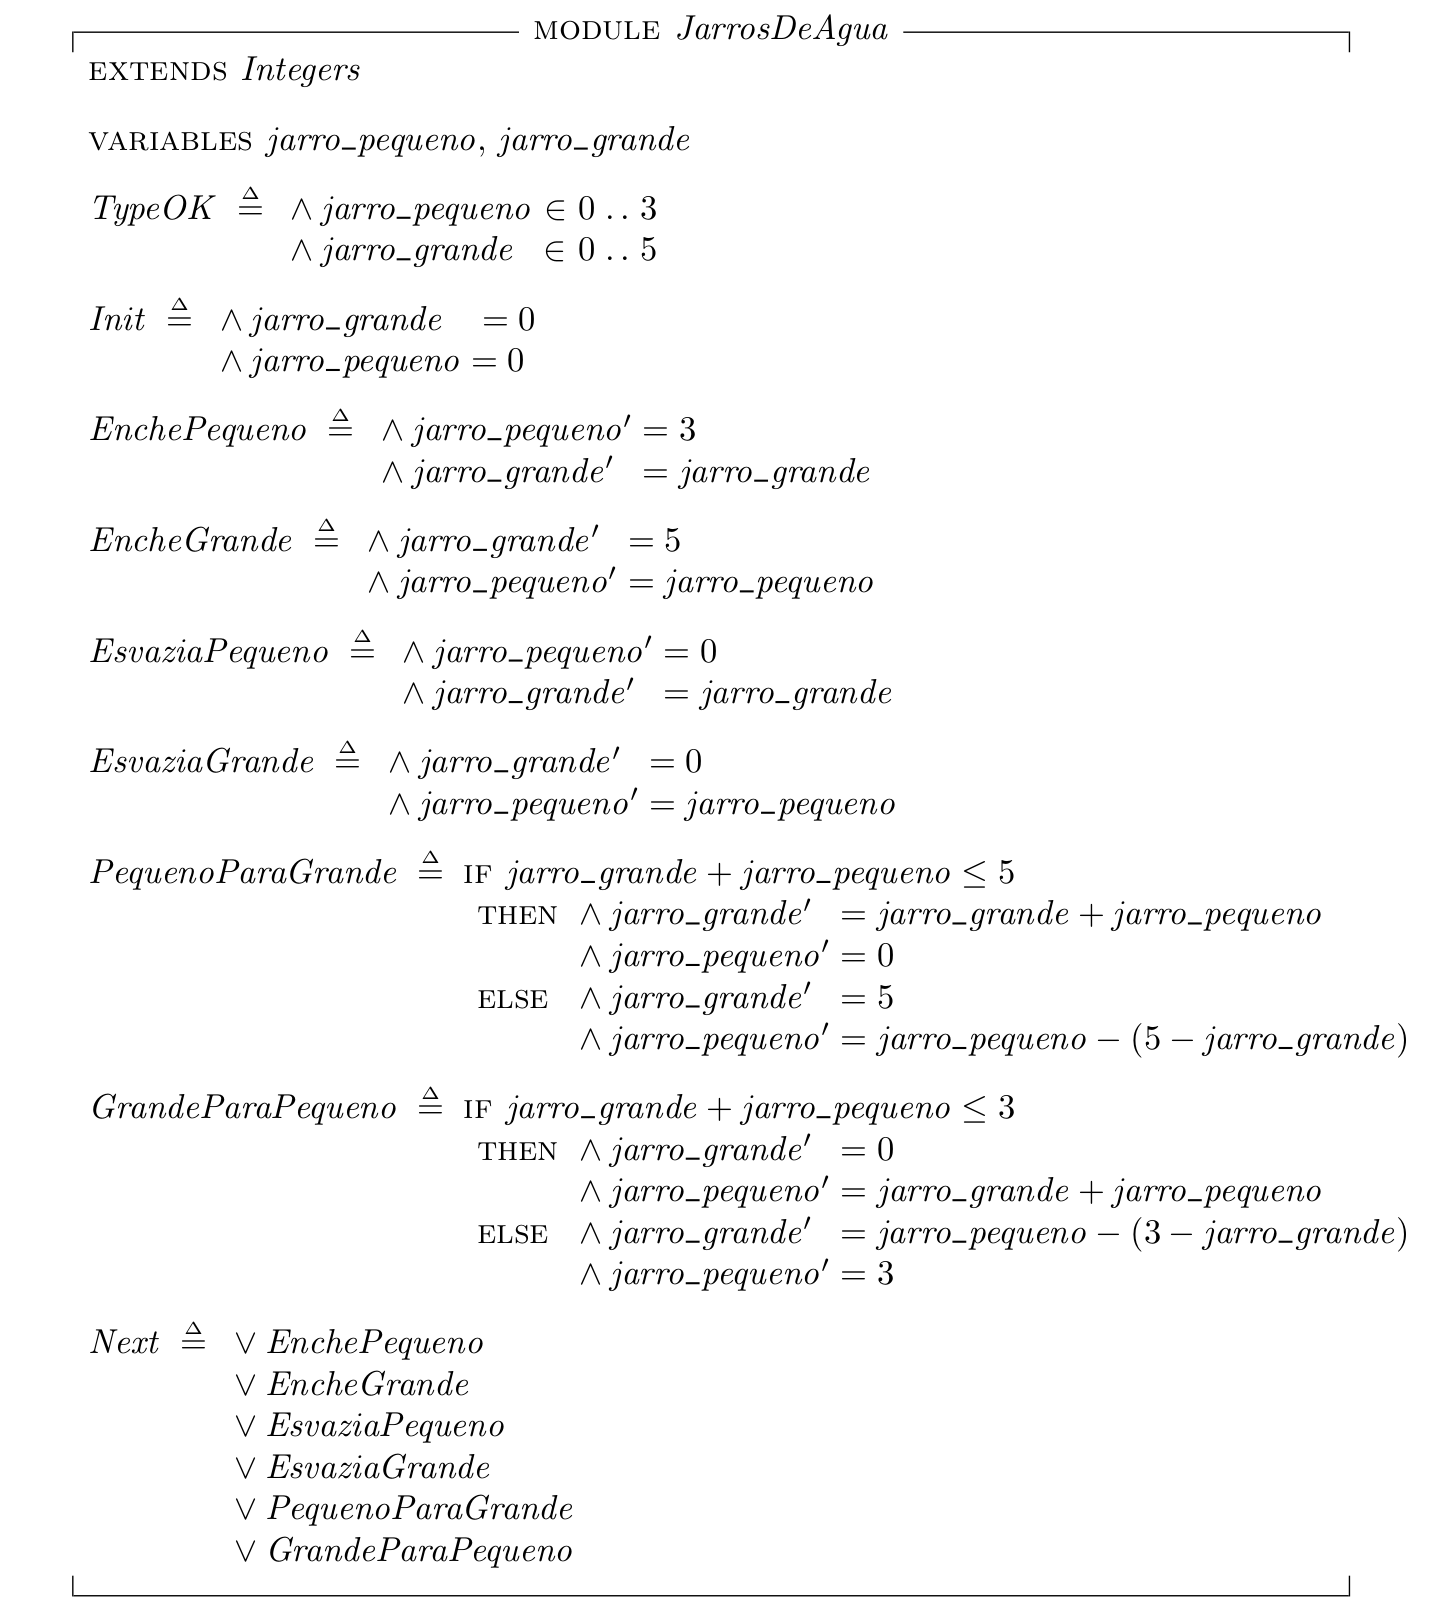
\includegraphics[width=\textwidth]{JarrosDeAgua.png}
  \caption{Especificação do problema dos Jarros de Água}
  \label{fig:ex1tla}
\end{figure}

Entendendo essa especificação no modelo de máquina de estado, é possível observar que as variáveis (\VARIABLES) são propriedades que variam nos estados, de forma que o conjunto com todas as combinações dos valores possíveis para cada uma das variáveis forma o conjunto de estados da máquina. Um estado desse sistema seria $jarro\_pequeno = 0, jarro\_grande = 1$. Na definição $Init$, é especificada uma fórmula que determina estados iniciais válidos - o que, nesse caso, é apenas o estado onde todas as variáveis tem valor 0.

As seis definições seguintes representam as transições através de fórmulas transicionais. Em cada uma delas, as variáveis com o símbolo de linha representam os valores no estado seguinte, e sempre precisam ser definidas. Na transição $EnchePequeno$, o valor de $jarro\_grande$ se mantém o mesmo entre os estados atual e seguinte, mas é necessário explicitar isso com $jarro\_grande' = jarro\_grande$. Essa necessidade vem da aproximação da sintaxe de \TLA com a matemática, onde não existe efeito colateral e, portanto, o valor da variável $jarro\_grande$ não propagaria de um estado para outro.

É possível, sintaticamente, utilizar a informação das variáveis do estado atual para definir o estado seguinte - não é necessário definir exaustivamente transições para todas as combinações de variáveis. Dessa forma, as fórmulas transicionais definidas representam transições para vários estados do sistema. Cada transição da especificação do problema dos jarros pode ser aplicada nos em qualquer um dos estados, isto é: $(jarro\_pequeno = 0, jarro\_grande = 0), (jarro\_pequeno = 0, jarro\_grande = 1), \dots$.

No sentido de aproveitar informações do estado atual, é possível utilizar condicionais, como nas fórmulas $PequenoParaGrande$ e $GrandeParaPequeno$. Com isso, é fácil definir transições diferentes para conjuntos de estados com propriedades diferentes. Na definição de $PequenoParaGrande$, os estados que atualmente possuem 5 litros ou menos de água nos jarros em total recebem uma transição para um estado onde o jarro pequeno está vazio. Já os estados que possuem mais de 5 litros de água recebem uma transição para um estado onde o jarro grande está cheio.

Ao fim dessa especificação, em $Next$, é definida a \textit{next state function} (função de próximo estado), na qual são declaradas as fórmulas transicionais do sistema, incluindo qualquer composição dessas fórmulas que possa levar um estado a outro. No caso do problema dos jarros, apenas é definido que qualquer transição pode ser utilizada para obter um novo estado.

As definições $Init$ e $Next$ são buscadas pelo \textit{model checker} TLC na construção da máquina de estados. É possível renomear essas definições, mas é preciso informar ao TLC os novos nomes para o estado inicial e a \textit{next state function}. A especificação - chamada $Spec$ - é descrita a partir dessas definições com a seguinte fórmula  temporal:

\[Spec \defeq Init \land \square [Next]_{vars}\]

Onde $vars$ é uma tupla contendo todas as variáveis. Com essa especificação, o sistema está definido. As operações permitidas e as variáveis relevantes foram descritas e, a partir do estado inicial, cada passo do sistema pode ser executado a partir de uma das seis diferentes fórmulas transicionais. Essas informações são suficientes para o TLC fazer verificações sobre o sistema, é apenas necessário definir tais verificações.

A definição $TypeOK$ na especificação apresentada pode ser utilizada para verificar os tipos desse sistema. Ela define que a variável $jarro\_pequeno$ é sempre um inteiro entre 0 e 3, e a variável $jarro\_grande$ é sempre um inteiro entre 0 e 5. Ou seja, $TypeOK$ será verdadeiro se e somente se os valores das variáveis estiverem de acordo com essas restrições. Isso não é uma verificação em si, e sim uma definição. Para que essa definição seja verificada em todos os estados alcançáveis pelo sistema, é necessário adicioná-la como uma invariante do modelo. Como uma invariante, o valor dela não deve ser modificado em nenhum estado da execução. Já que o estado inicial definido em $Init$ faz $TypeOK$ verdadeiro, ao colocar essa invariante, todos os estados devem fazer $TypeOK$ verdadeiro, ou o TLC retornará um erro. $TypeOk$ pode ser definido como uma invariante através do teorema:

\[\THEOREM Spec \implies \square (TypeOK)\]

Outra propriedade interessante de ser verificada para esse problema antes da implementação de um programa para resolvê-lo é a possibilidade de resolução, isto é, se é possível alcançar um estado onde onde o jarro maior contém 4 litros de água. Para isso, define-se uma invariante para o predicado $jarro\_grande\ \backslash= 4$, que não será satisfeita. Como esse predicado é verdadeiro para o estado inicial, o fato de ele não ser satisfeito significa que, em algum momento da execução, o predicado foi falso, ou seja, $jarro\_grande = 4$. Adicionando essa invariante, um possível teorema seria:

\[\THEOREM Spec \implies \square (TypeOK \land jarro\_grande\ \backslash= 4)\]

O TLC, ao encontrar uma execução que insatisfaz a invariante, traz a sequência de transições que levam ao estado onde o predicado é falso, o que, no caso do simples problema dos jarros, é a solução buscada.

Esse exemplo é apresentado com o intuito de demonstrar a estrutura da especificação de um sistema e o funcionamento das invariantes. A seguir, é proposto um exemplo com especificações de um sistema real e de um programa que atua nele.

\section{Exemplo 2 - Transações em Bancos de Dados}

Já em um contexto de um problema real de sistemas concorrentes, define-se uma especificação para o problema da consistência das transações em bancos de dados. Esse é um problema clássico onde, dado um conjunto de gerenciadores de recursos fazendo operações sobre um mesmo banco, um gerenciador só pode cometer (fazer a ação \textit{commit}) se todos os outros estiverem preparados para cometer, e se algum gerenciador quiser abortar, então todos devem abortar.

Na Figura \ref{fig:ex2tla}, encontra-se uma especificação para um sistema de transações consistente. Ela não apresenta uma proposta de solução para o problema, e sim traz uma descrição formal do que significa ser consistente. Uma especificação de uma solução para o problema deve implementar essa especificação.



\begin{figure}
  \centering
  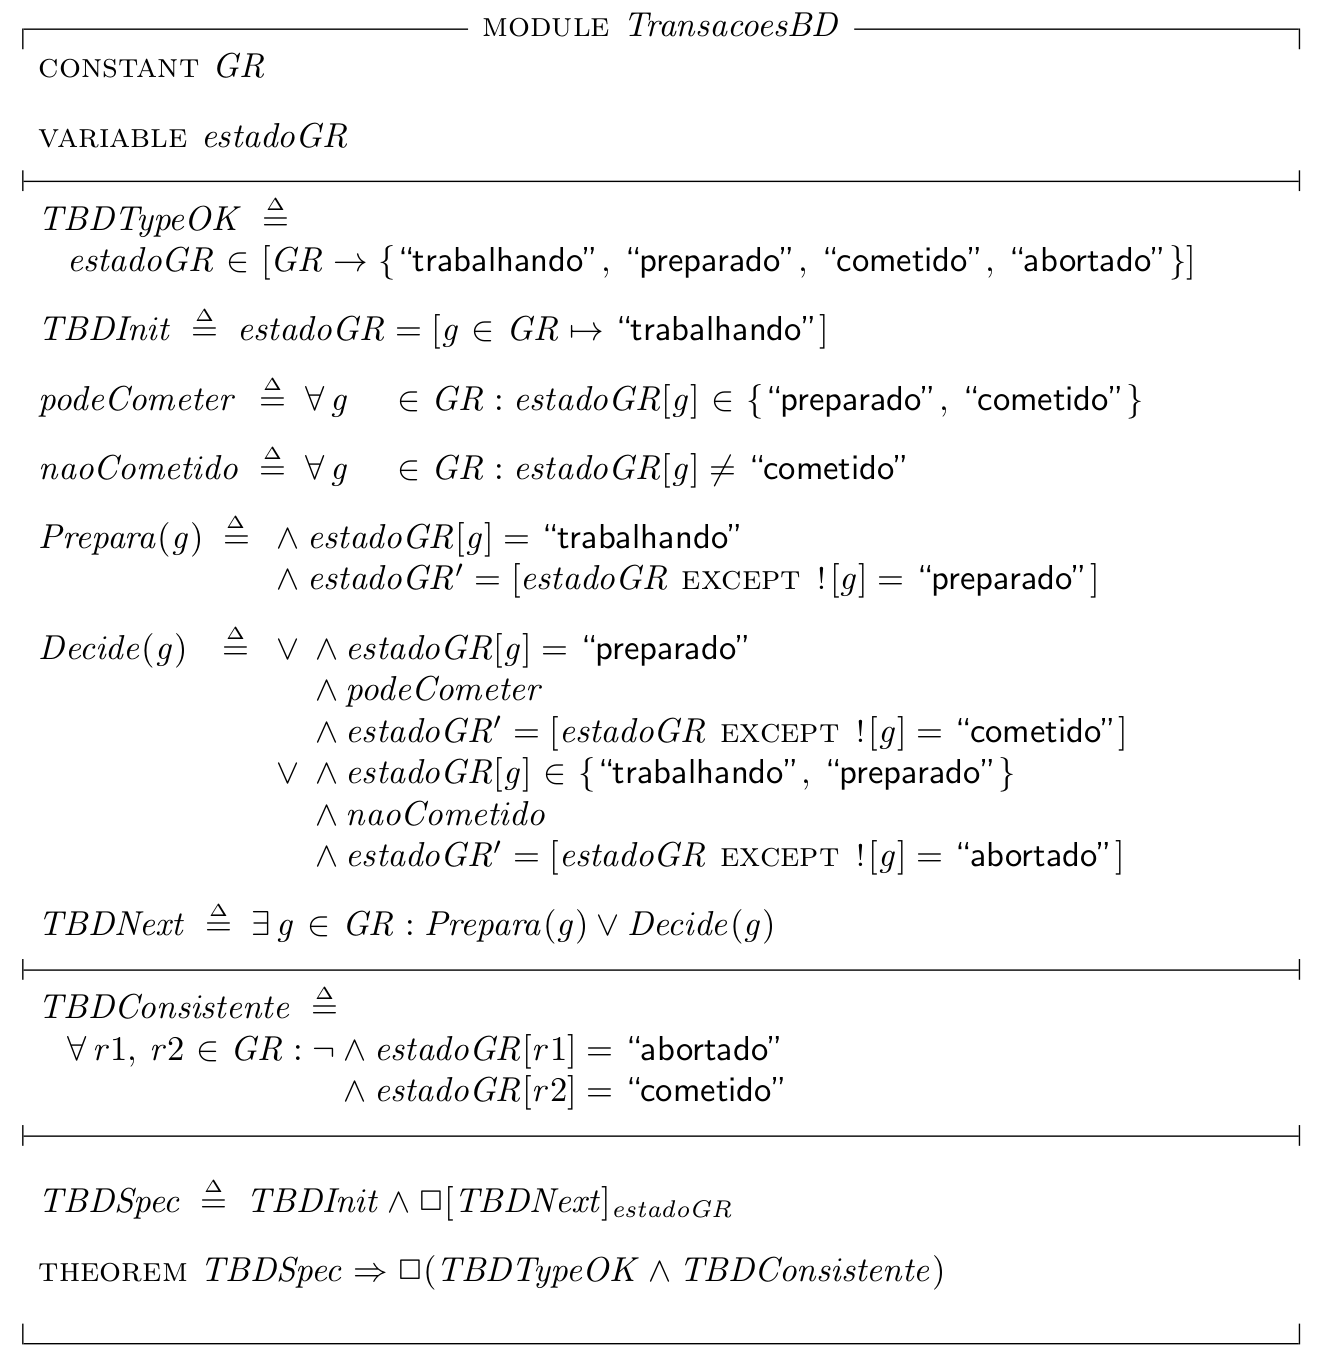
\includegraphics[width=\textwidth]{TransacoesBD.png}
  \caption{Especificação do problema das Transações}
\label{fig:ex2tla}
\end{figure}
